\documentclass{article}
\usepackage{tikz}
\usetikzlibrary{calc}

\tikzset{
	right angle quadrant/.code={
		\pgfmathsetmacro\quadranta{{1,1,-1,-1}[#1-1]}     % Arrays for selecting quadrant
		\pgfmathsetmacro\quadrantb{{1,-1,-1,1}[#1-1]}},
	right angle quadrant=1, % Make sure it is set, even if not called explicitly
	right angle length/.code={\def\rightanglelength{#1}},   % Length of symbol
	right angle length=2ex, % Make sure it is set...
	right angle symbol/.style n args={3}{
		insert path={
			let \p0 = ($(#1)!(#3)!(#2)$) in     % Intersection
			let \p1 = ($(\p0)!\quadranta*\rightanglelength!(#3)$), % Point on base line
			\p2 = ($(\p0)!\quadrantb*\rightanglelength!(#2)$) in % Point on perpendicular line
			let \p3 = ($(\p1)+(\p2)-(\p0)$) in  % Corner point of symbol
			(\p1) -- (\p3) -- (\p2)
		}
	}
}

\begin{document}
	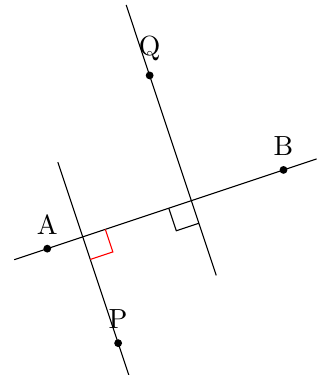
\begin{tikzpicture}[dot/.style={circle,inner sep=1pt,fill,label={#1},name=#1},
	extended line/.style={shorten >=-#1,shorten <=-#1},
	extended line/.default=1cm]
	
	\node [dot=A] at (0,0) {};
	\node [dot=B] at (3,1) {};
	\node [dot=P] at (0.9,-1.2) {};
	\node [dot=Q] at (1.3,2.2) {};
	
	\draw [extended line=0.5cm] (A) -- (B);
	\draw [extended line] ($(A)!(P)!(B)$) -- (P);
	
	
	\draw [red,right angle symbol={A}{B}{P}];
	
	\draw [extended line,right angle quadrant=3,right angle symbol={A}{B}{Q}] ($(A)!(Q)!(B)$) -- (Q);
	\end{tikzpicture}
\end{document}